\documentclass{article} 
\usepackage{amsmath} 
\usepackage{amssymb} 
\usepackage{amsthm} 
\usepackage[margin=0.2in]{geometry} 
\usepackage{hyperref} 
\usepackage{physics} 
\usepackage{tikz} 
\usepackage{mathtools}
\usepackage{graphicx}\graphicspath{{./images/}}
\mathtoolsset{showonlyrefs} 
\theoremstyle{definition} 
\newtheorem{theorem}{Theorem}[section] 
\newtheorem{corollary}{Corollary}[theorem] 
\newtheorem{lemma}[theorem]{Lemma} 
\newtheorem{definition}{Definition}[section] 

\author{Connor Duncan}
\date{\today}

\title{notes-10-14-2019}
\begin{document}
\abstract{A single document copy of these notes, as well as a mirror of every note, can be found at \url{connorduncan.xyz/notes}}
\section{Quantum Scattering} \subsection{Classical Scattering} We want first to compare quantum with classical scattering. Consider the following setup, with some flux of particles coming into a sheet at a flux $j_{\mathrm{in}}=\pdv{I}{A}$. We have the outgoing flux per steradian, $\pdv{I}{\Omega}$, and want t ocompute the ratio \begin{equation} \pdv{\sigma}{\Omega}=\frac{\pdv{I}{\Omega}}{\pdv{I}{A}} \end{equation} We will consier our target to exhibit some central potential $V(r)$. The classical model should project that it will behave as follows\footnote{this is just copy-pasted from my 105 notes, so the notation might not be exactly the same.} \begin{center} 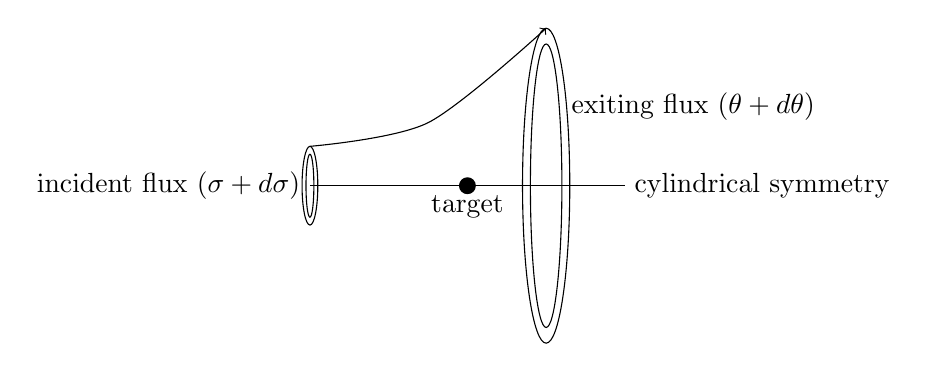
\begin{tikzpicture} \draw[->] plot [smooth] coordinates {(-2,0.5)(-0.5,0.8)(1,2)}; \draw (-2,0)--(2,0) node[anchor=west]{cylindrical symmetry}; \draw[fill] (0,0) ellipse (0.1) node[anchor=north]{target}; \draw (-2,0) ellipse (0.1 and 0.5) (-2,0) ellipse (0.05 and 0.4) node[anchor=east]{incident flux $(\sigma+d\sigma)$}; \draw (1,0) ellipse (0.3 and 2) (1,0) ellipse (0.2 and 1.8) (1.2,1)node[anchor=west]{exiting flux ($\theta+d\theta$)}; \end{tikzpicture} \end{center} We're going to consider \begin{center} \includegraphics[width=0.5\textwidth]{classical-scatter} \end{center} which has \begin{equation} dI=\pdv{n}{t}=j_\mathrm{in}d\sigma=j_{\mathrm{in}}\pdv{\sigma}{\Omega}d\Omega \end{equation} where \begin{equation} \pdv{\sigma}{\Omega}=\frac{\partial I/\partial\Omega}{j_\mathrm{in}} \end{equation} which gives our previous result! We can attempt to characterise this differential cross section by the distance $b$ from the axis of symmetry of the incoming particle. \begin{center} \begin{tikzpicture} \draw[->] plot [smooth] coordinates {(-2,0.5)(-0.5,0.8)(1,2)}; \draw[dashed] (-2,0)--(2,0); \draw[<->] (-1.8,0)--(-1.8,0.6); \node (b) at (-1.6,0.3) {$b$}; \draw[fill] (0,0) ellipse (0.1) node[anchor=north]{target}; \draw[->] plot [smooth] coordinates {(-2,-0.5)(-0.5,-0.8)(1,-2)}; \end{tikzpicture} \end{center} We can consider $d\sigma$ to be a small piece of area, $d\sigma=bdbd\phi$. This gives that $dI=jd\sigma=jdbd\phi=j\pdv{\sigma}{\Omega}d\Omega$, which gives (after cancelling the $d\phi$ from $d\Omega=sin\theta d\phi d\theta$), so we have \begin{equation} \pdv{\sigma}{\Omega}=\frac{b}{\sin\theta}\pdv{b}{\theta} \end{equation} This is a pretty niche equation though. We have it in terms of $b,$ the impact parameter, $E$, the precise energy that we shoot it at. We want a more general quantity, which we call $\sigma_T$, the total cross section. We're going to integrate over a sphere surrounding the target. We take \begin{equation} \sigma_T=\iint_Vd\Omega\pdv{\sigma}{\Omega} \end{equation} \begin{center} 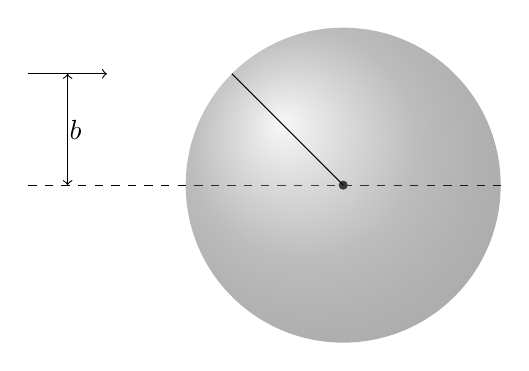
\begin{tikzpicture} \draw[->] (-4,{2/sqrt(2)})--(-3,{2/sqrt(2)}); \draw[fill] (0,0) ellipse (0.05); \draw[dashed] (-4,0)--(2,0); \draw[<->] (-3.5,0)--(-3.5,{2/sqrt(2)}); \node (b) at (-3.4,{1/sqrt(2)}) {$b$}; \shade[ball color=gray, opacity =0.4] (0,0) circle (2); \draw (0,0)--(-{1/sqrt(2)*2},{1/sqrt(2)*2}); \end{tikzpicture} \end{center} I'll try and finish the pretty drawing later. \begin{center} \includegraphics[width=0.5\textwidth]{classical-hard-sphere} \end{center} We can compute \begin{equation} \sigma_T=\int\pdv{\sigma}{\Omega}d\Omega=\frac{R^2}{4}\int d\Omega=\frac{4\pi R^2}{4}=\pi R^2 \end{equation} For more on this topic, check out Chapter 14 of Taylor\footnote{Not reccomended by altman, I just like the book lol. He said he would post a summary.}. Altman is going to move on to quantum though. \subsection{Beginning Quantum Scattering} We're going to look for eigenvalues of the schroedinger equation, where we have \begin{equation} \left[\frac{-\hbar}{2m}\nabla^2+V(r)\right]\psi(r)=E\psi(r) \end{equation} We're going to begin by looking for solutions of the form \begin{equation} \psi(r)=\psi_\mathrm{inc}(r)+\psi_\mathrm{sc}(r) \end{equation} where $\psi_\mathrm{inc}$ is an incident plane wave, and $\psi_\mathrm{sc}$ is the scattered component, where \begin{align} \psi_\mathrm{inc}=e^{ikz} && \psi_\mathrm{sc}=f(\theta,\phi)\frac{e^{ikr}}{r} \end{align} We make the switch to spherical coordinates, in the following manner \begin{equation} \vec{r}=(\sin\theta\cos\phi|r|,\sin\theta\sin\phi|r|,\cos\theta|r|) \end{equation} Eventually, we're going to find for various cylindrical symmetries that $\phi$ will drop out of our function $f$.
\end{document}
